\documentclass[pdftex, 12pt,a4paper,oneside]{report}
\usepackage{amsmath}
\usepackage{amsfonts}
\usepackage{amssymb}
\usepackage{times}
\usepackage{graphicx}
\usepackage{caption}
\usepackage{subcaption}
\begin{document}
\begin{center}
\noindent\makebox[\linewidth]{\rule{\textwidth}{1pt}}
\textbf{CRISM Despiking for GALE IMAGES}\\
\textbf{September 26$^{th}$, 2013}
\noindent\makebox[\linewidth]{\rule{\textwidth}{1pt}}
\end{center}

\textbf{Column Average Based Noise Reduction}\\
\\We start with the TRR3, which has been pre-corrected for atmosphere using the Lambertian Albedo-based methods.\\ 
\\Consider an Hyperpsectral image (HSI) $Y$ with '$r$' rows, '$c$' columns and '$b$' bands. A pixel corresponds to a spatial location, i.e. ($Y(i,j,:)$), while a spectel is a the value at a given band for a given pixel i.e. ($Y(i,j,k)$). The signal at each pixel in $Y$ can be modeled as a combination of the signal corresponding to the minerals present at that location, some detector specific noise and other noise processes. That is we can represent the signal in a band $k$ as:- 
\begin{equation}
Y(i,j,k) = S(i,j,k) + n_d(i,j,k) + n(i,j,k)
\label{1}
\end{equation}
Where $S(i,j,k)$ is the useful signal we are looking for, $n_d$ is the detector specific noise , $n$ represents the effect of random noise processes. Now since every pixel in a column(samples) of Y are measured using the same detector(s) they must all suffer from similar distortions common to the column. In simplest terms we approximate the column dependent as a scaled version of some fixed detector-specific noise profile ($\tilde{\mu_{y}}(k)$). We can now rewrite Eqn. ($\ref{1}$) as:- 
\begin{equation}
Y(i,j,k) = S(i,j,k) + \alpha(i,j)\tilde{\mu}_y(k) + n(i,j,k)
\label{2}
\end{equation}
Where $\alpha(i,j)$ is scaling factor proportional to the strength of the signal. \\
\\If we find the average spectra for a given column  in the image the average column spectel $\mu_y (k)$, this will be a combination of the average mineral spectra in the column and the noise profile (Assuming that the other random noise has zero mean).Since we think that mineral spectra will be smooth, we smoothed the average mineral spectra using splines to seperate the portion of the signal depending on the minerals in the scene from the detector based distortions. In effect we assume that ($\mu_{y}(k)$) can be broken into: -
\begin{equation}
\mu_{y} = \bar{\mu}_y (k) + \tilde{\mu}_y (k)
\label{3}
\end{equation}
where $\bar{\mu}_y (k)$ is the estimated average mineral signal and $\tilde{\mu}_y (k)$  is the estimated signal based noise/distortion. We can use the estimated noise signal to correct the signal in the image as
\begin{equation}
\tilde{S}(i,j,k) = Y(i,j,k) - \alpha(i,j) \tilde{\mu}_y (k)
\label{4}
\end{equation}

This column average based corrections seems to be quite successful in general in removing any remaining atmospheric distortions and also seems to generally reduces the noise in the signal.\\
\\
\textbf{Neighborhood Based Despiking for CRISM Images}\\
\\In CRISM images other than the atmospheric distortions and mixing the spectra are also affected significantly by distortions caused by the detectors. The distortions are often very local in nature and don't last more than a few pixels. Since these distortions are very local in the nature processes like the average in the previous section do not correct for these distortions. This is of great significance for the despiking process as very often neighboring pixels are highly similar in compositions and the shape of the neighboring pixels can be used to correct the shape of the distorted pixels in the image.\\ 
\\
In general the spikes/distortions manifest in the form high-frequency changes in the signal. The spikes are seen as sudden and narrow drops or jumps in the intensity. In general the spectels that are affected by such distortions have a larger difference to their immediate neighbors than other spectels. We attempt to capture the band-to-band for a given pixel difference using the intensity differential as: -

\begin{multline}
intDiff(i) = [(intensity(i) - intensity(i)|]) + ... (|intensity(i) - intensity(i))\\
\mu_{intDiff} = mean(intDiff), ~~mean~of~intDiff~for~the~pixel
\end{multline}

In general mineral spectra change quite smoothly and the amount of intensity changes consistently the sudden change maybe because of distortions. We select these spectels of sudden change as possible spike regions. In general if spectel has intDiff(i) that is more than 1.15 the $\mu_{intDiff}$ , those spectels are flagged as possible spike locations. Also in some cases the intensity differential is caused by the presence of spectral bands or some other spectral features. Once the spiky pixels are identified the algorithm attempts to interpolate through these distorted spectels in an attempt to better reveal the shape.But a simple interpolation might not correctly reproduce the spectral shape. Instead attempt to reproduce in this pixel the shape that other spectra in that range. We hope that since very often pixels are very similar to it's immediate neighbors that the shape of the neighbors would better reveal the shape of the mineral spectra in the region. This is also a good idea because if a spectel is incorrectly tagged as spike, but all it's neighbors have the same shape in the region then we reintroduce the original shape back into the spectra.\\
\\
\textbf{Results}
We applied the two steps mentioned above to two images from the CRISM dataset i.e FRT00017F45 and FRT00003FB9. In both images the methods were successful in rendering the signals easier to identify and also in reducing the noise present in the signal. 
\begin{figure*}[!ht]
        \centering
        \begin{subfigure}[b]{0.2\textwidth}
                \centering
                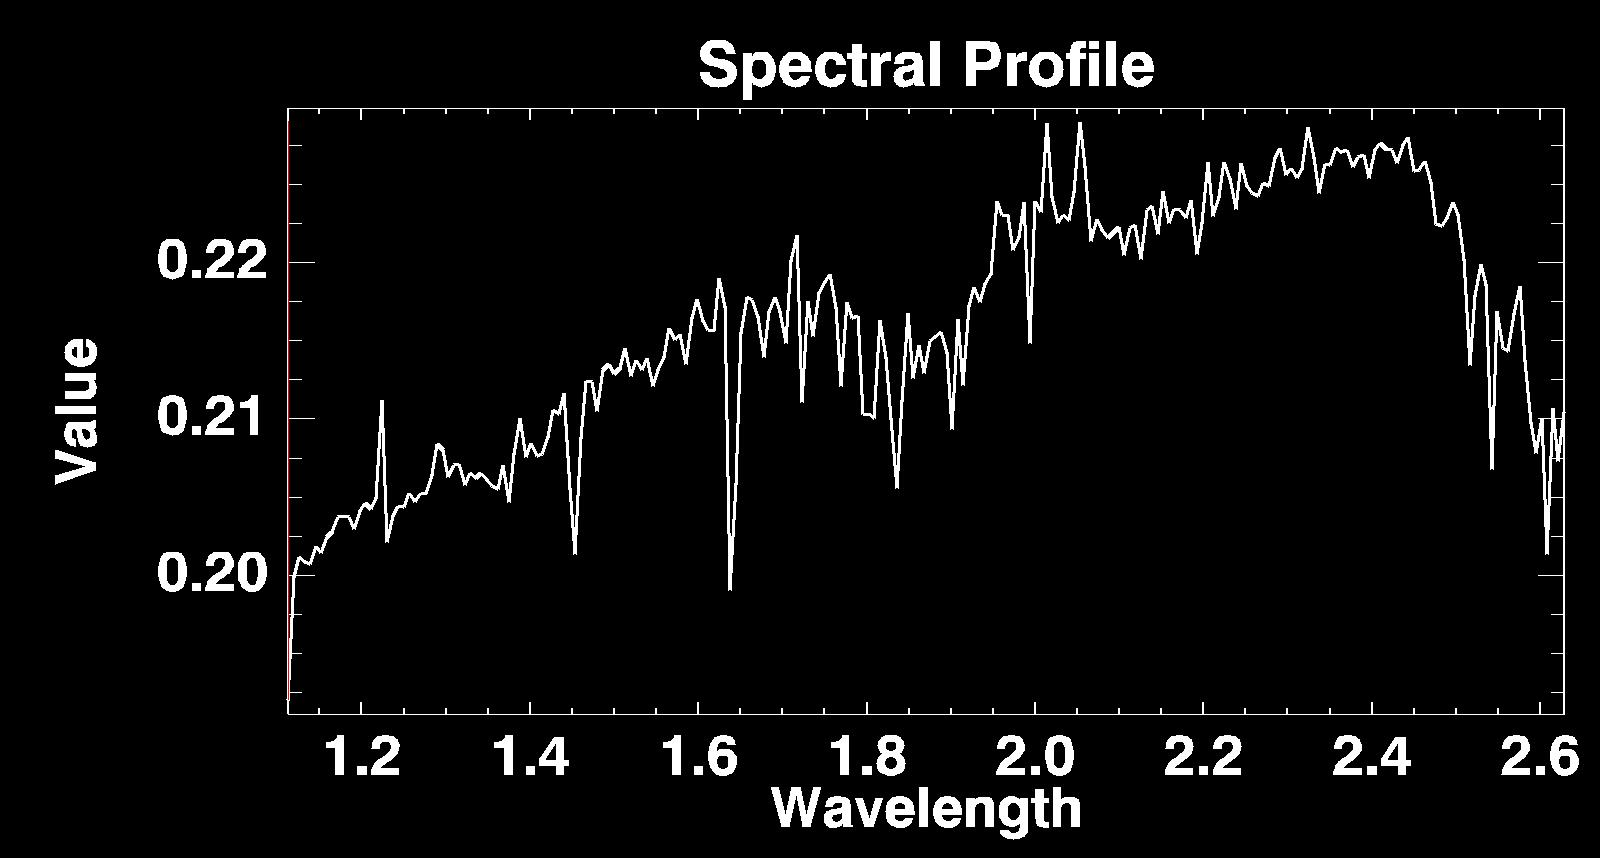
\includegraphics[width=\textwidth, height=1.5in]{orig17F45_328_343.jpg}
                \caption{The original pixel}
                \label{fig:origPix_1}
        \end{subfigure}
        \qquad
        \quad
		\begin{subfigure}[b]{0.2\textwidth}
                \centering
                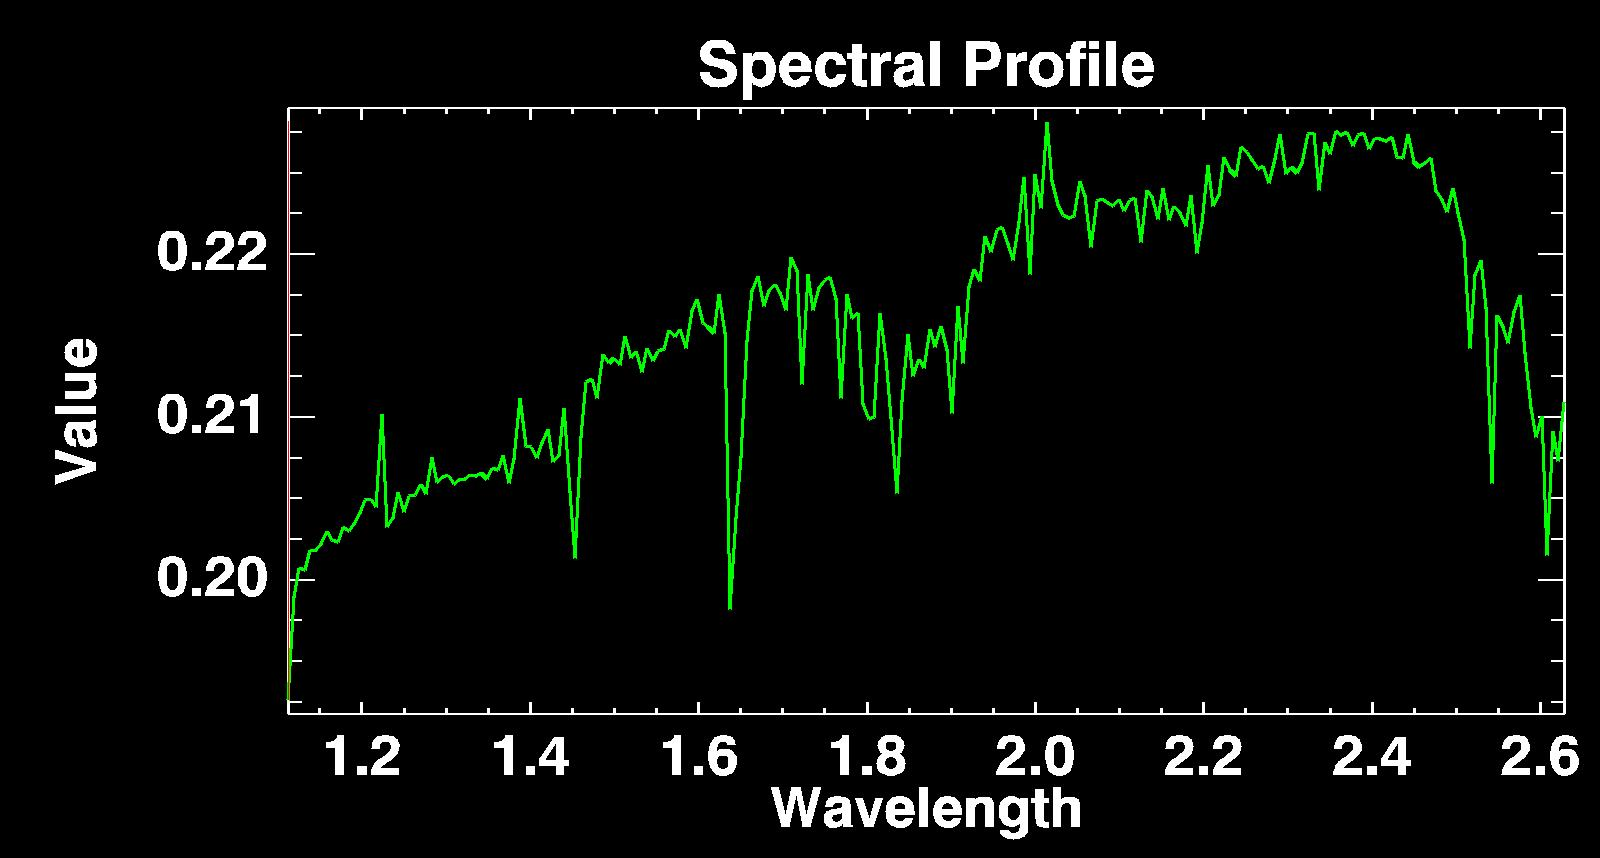
\includegraphics[width=\textwidth, height=1.5in]{avgCorr17F45_328_343.jpg}
                \caption{column average correction}
                \label{fig:avgCorr_1}
        \end{subfigure}   
        \qquad    
        \quad
        \begin{subfigure}[b]{0.2\textwidth}
                \centering
                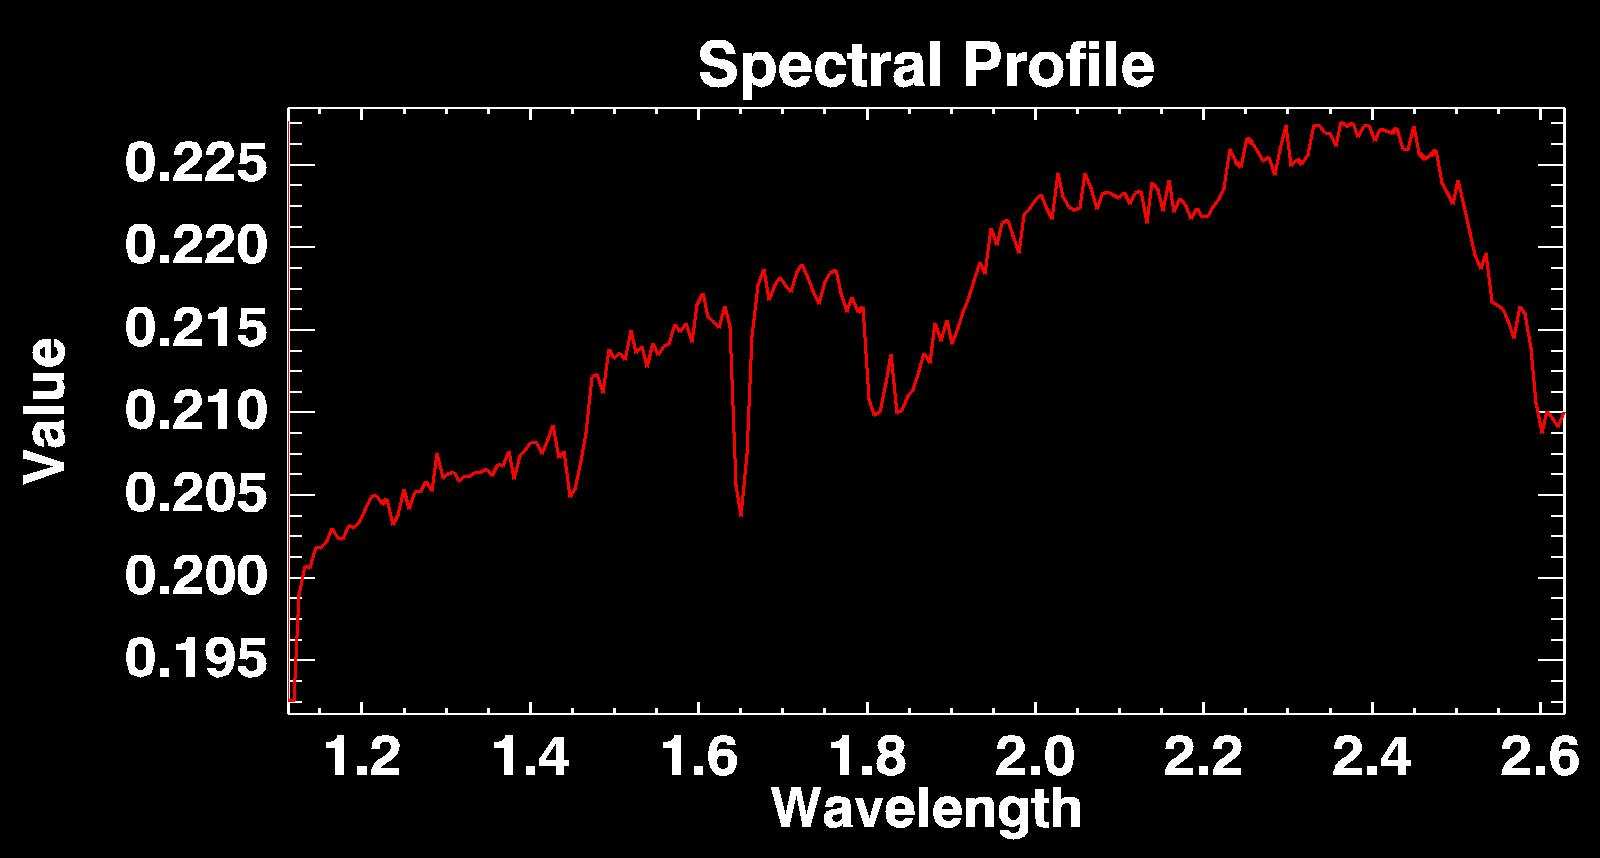
\includegraphics[width=\textwidth, height=1.5in]{dspkavgCorr17F45_328_343.jpg}
                \caption{After final Despiking}
                \label{fig:dspkCorr_1}
        \end{subfigure}%
        ~ 
        
        \caption{Effect the column average correction and despiking for 17F45 pixel at sample = 328 and line = 343.}
               
\end{figure*} 

\begin{figure*}[!ht]
        \centering
        \begin{subfigure}[b]{0.2\textwidth}
                \centering
                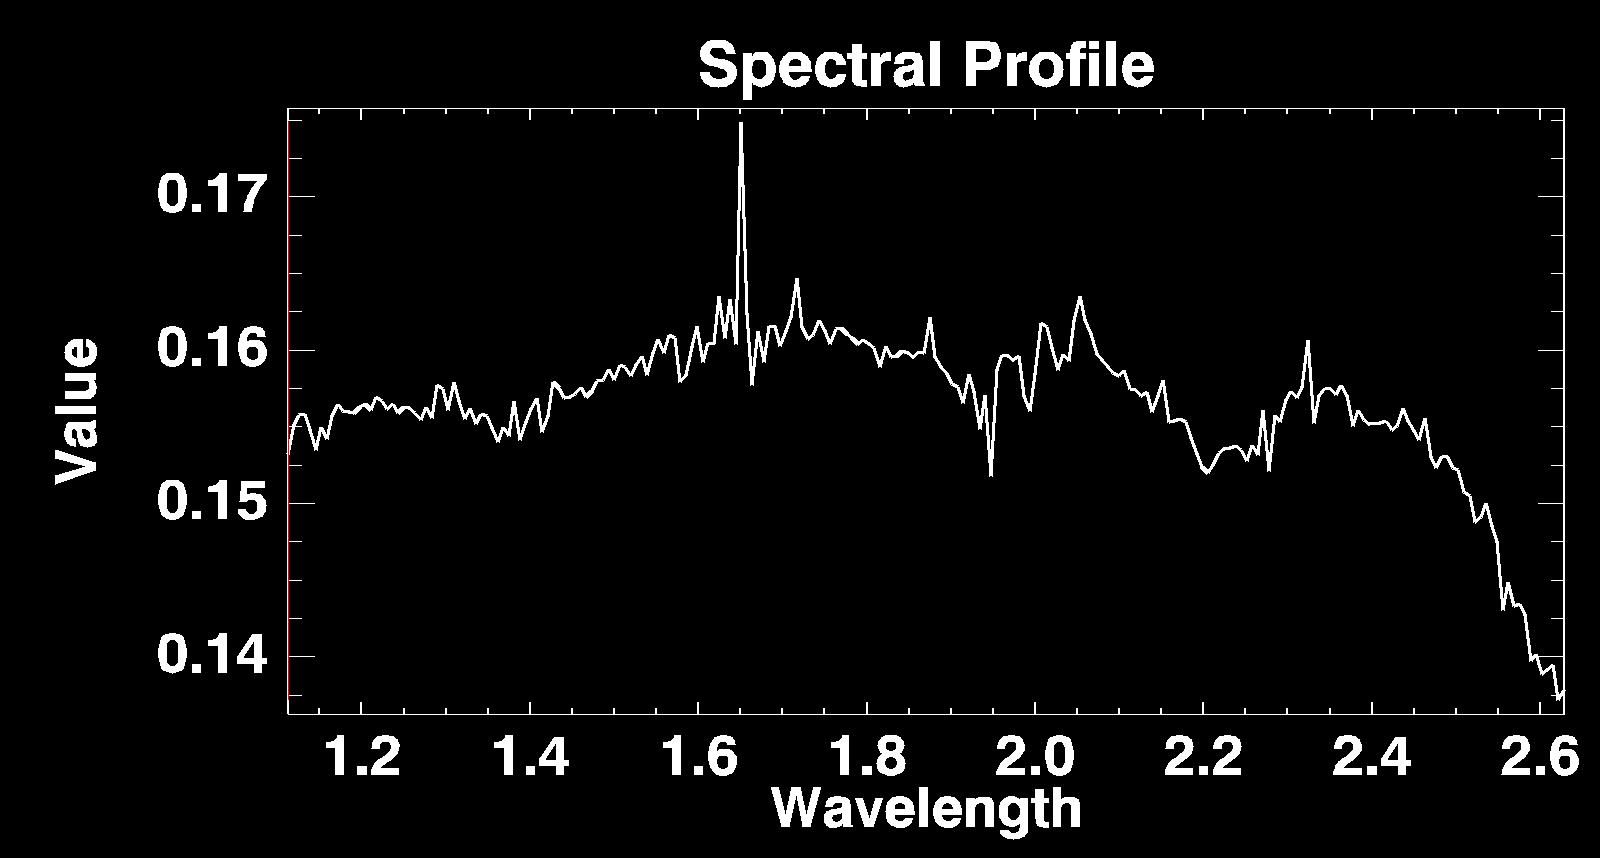
\includegraphics[width=\textwidth, height=1.5in]{orig17F45_349_200.jpg}
                \caption{The original pixel}
                \label{fig:origPix_1}
        \end{subfigure}
        \qquad
        \quad
		\begin{subfigure}[b]{0.2\textwidth}
                \centering
                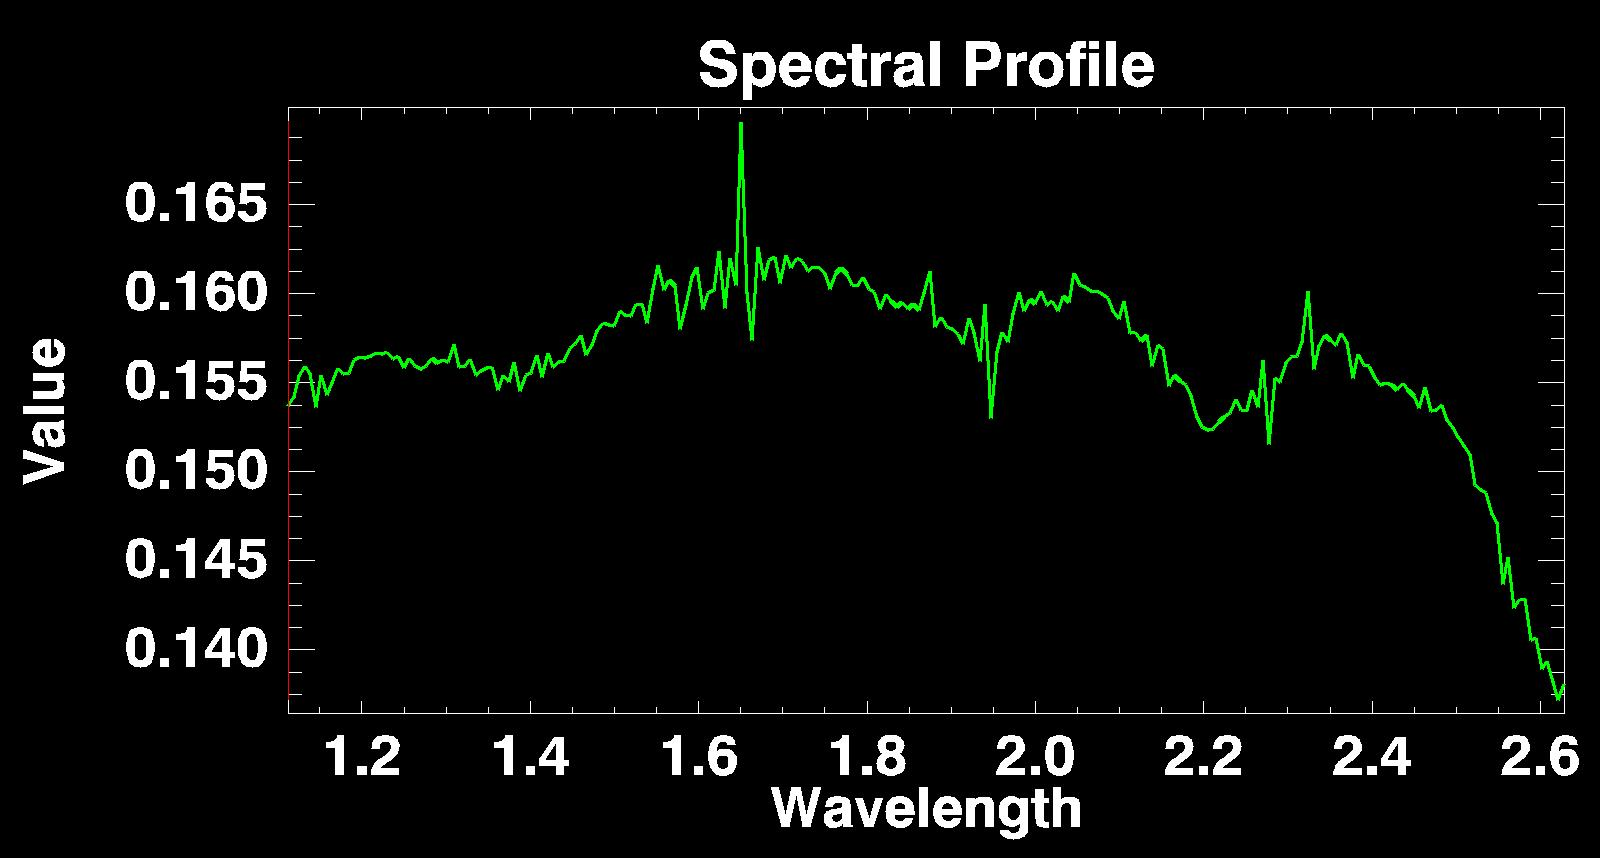
\includegraphics[width=\textwidth, height=1.5in]{avgCorr17F45_349_200.jpg}
                \caption{column average correction}
                \label{fig:avgCorr_1}
        \end{subfigure}   
        \qquad    
        \quad
        \begin{subfigure}[b]{0.2\textwidth}
                \centering
                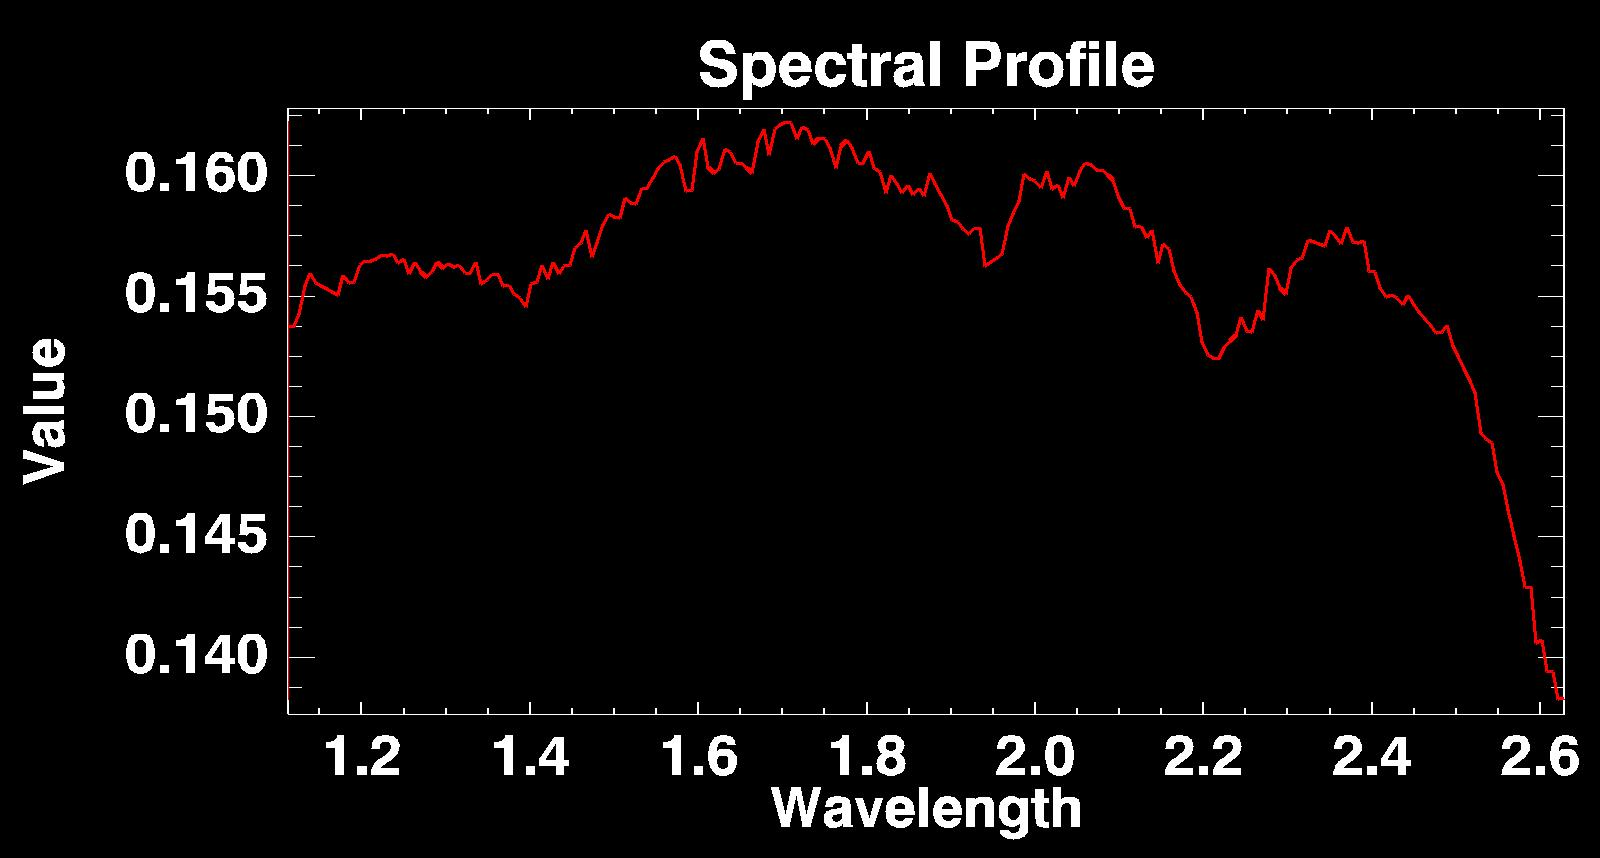
\includegraphics[width=\textwidth, height=1.5in]{dspkavgCorr17F45_349_200.jpg}
                \caption{After final Despiking}
                \label{fig:dspkCorr_1}
        \end{subfigure}%
        ~ 
        
        \caption{Effect the column average correction and despiking for 17F45 pixel at sample = 348 and line = 200.}
               
\end{figure*} 

\begin{figure*}[!ht]
        \centering
        \begin{subfigure}[b]{0.2\textwidth}
                \centering
                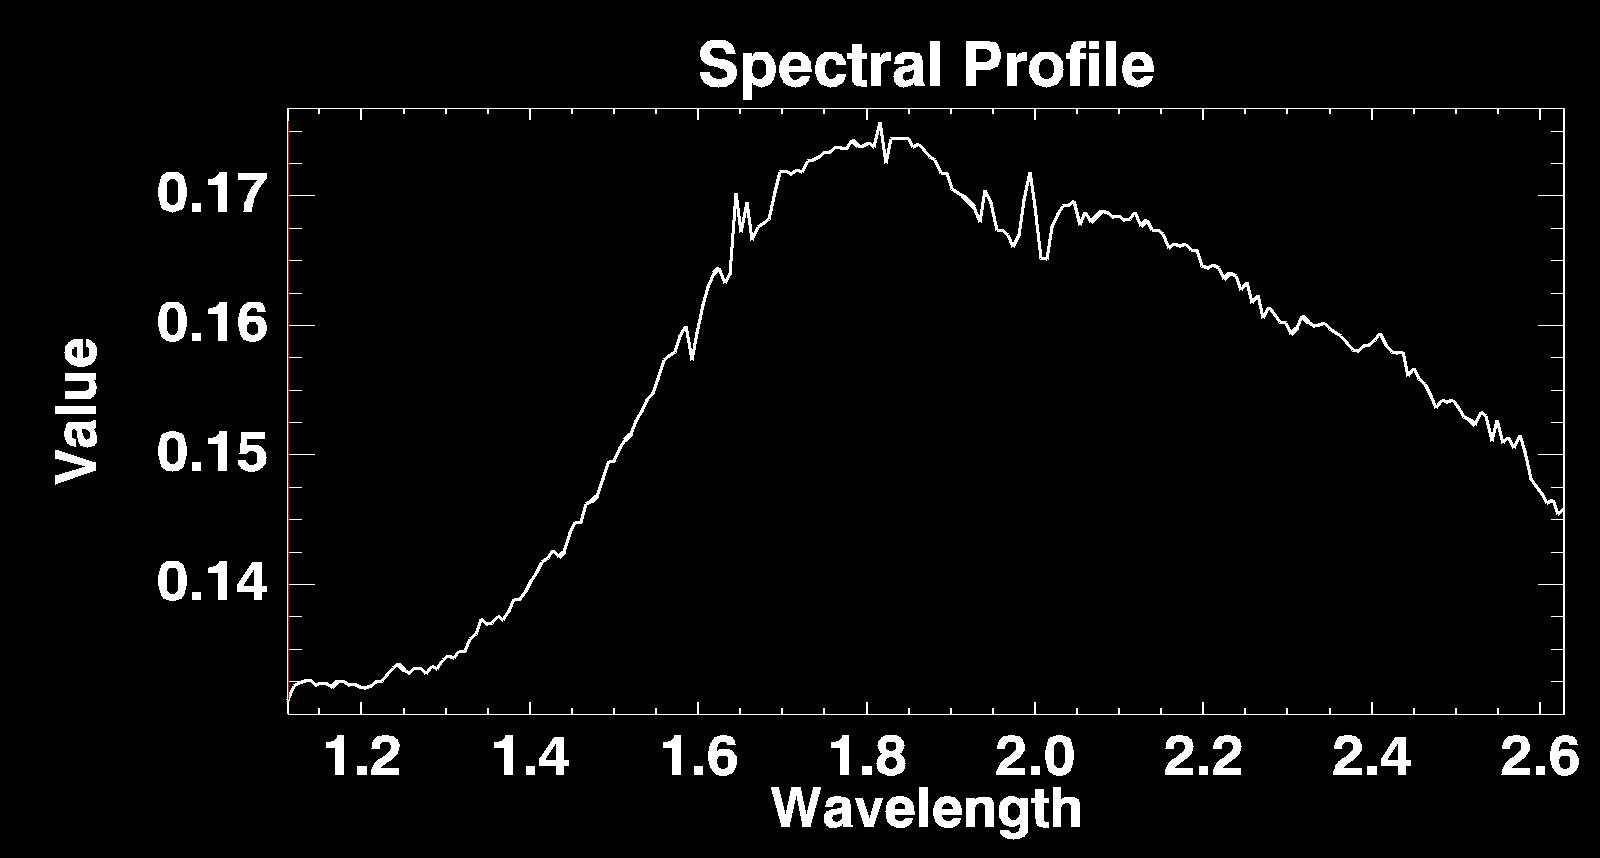
\includegraphics[width=\textwidth, height=1.5in]{orig3FB9_201_200.jpg}
                \caption{The original pixel}
                \label{fig:origPix_1}
        \end{subfigure}
        \qquad
        \quad
		\begin{subfigure}[b]{0.2\textwidth}
                \centering
                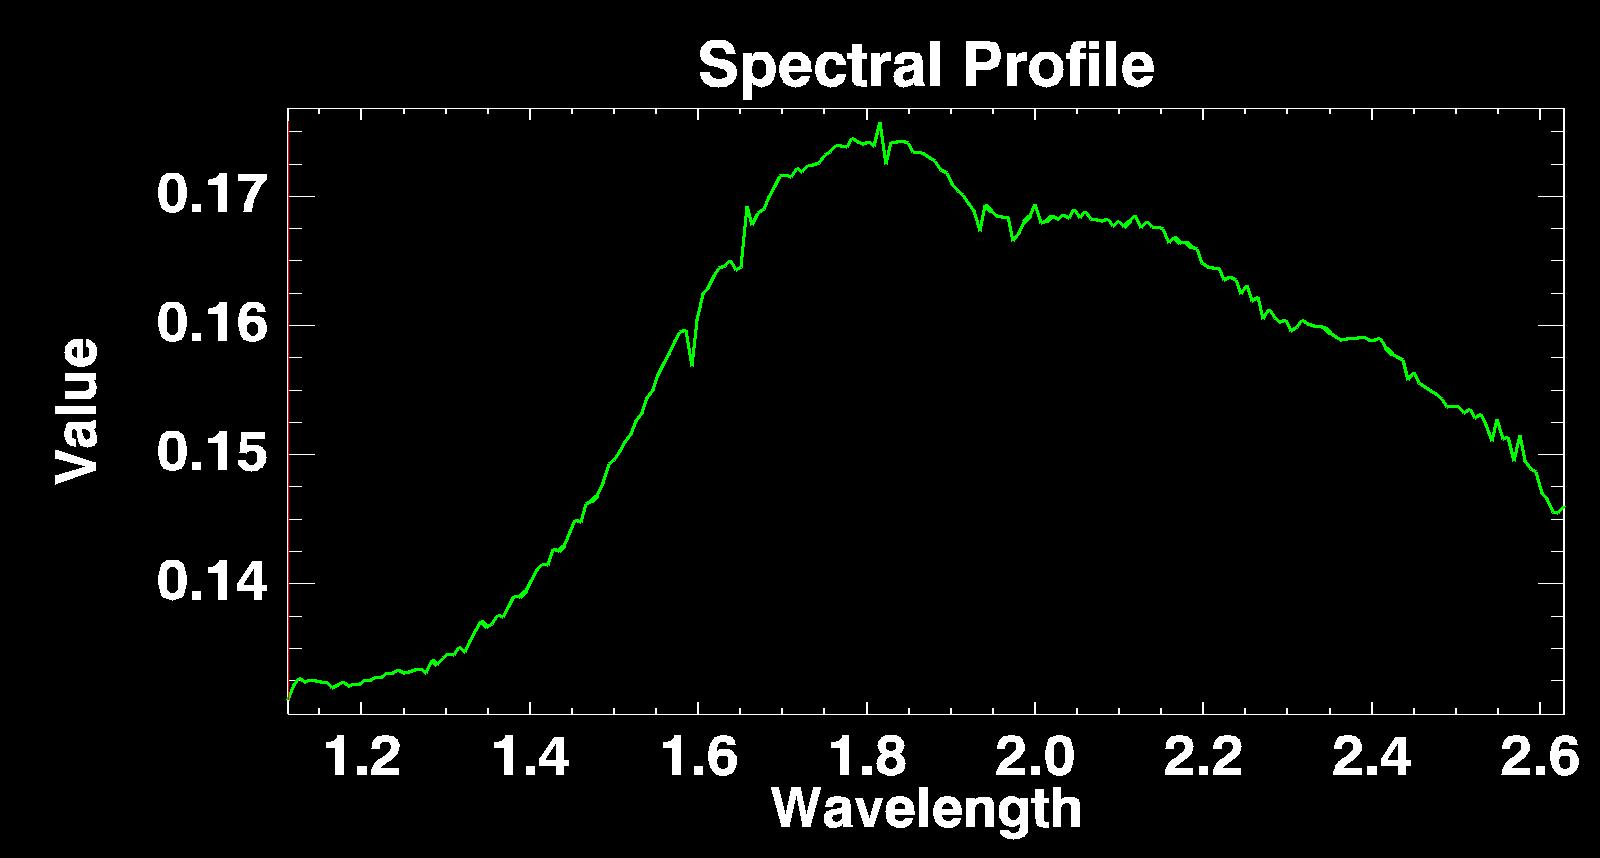
\includegraphics[width=\textwidth, height=1.5in]{avgCorr3FB9_201_200.jpg}
                \caption{column average correction}
                \label{fig:avgCorr_1}
        \end{subfigure}   
        \qquad    
        \quad
        \begin{subfigure}[b]{0.2\textwidth}
                \centering
                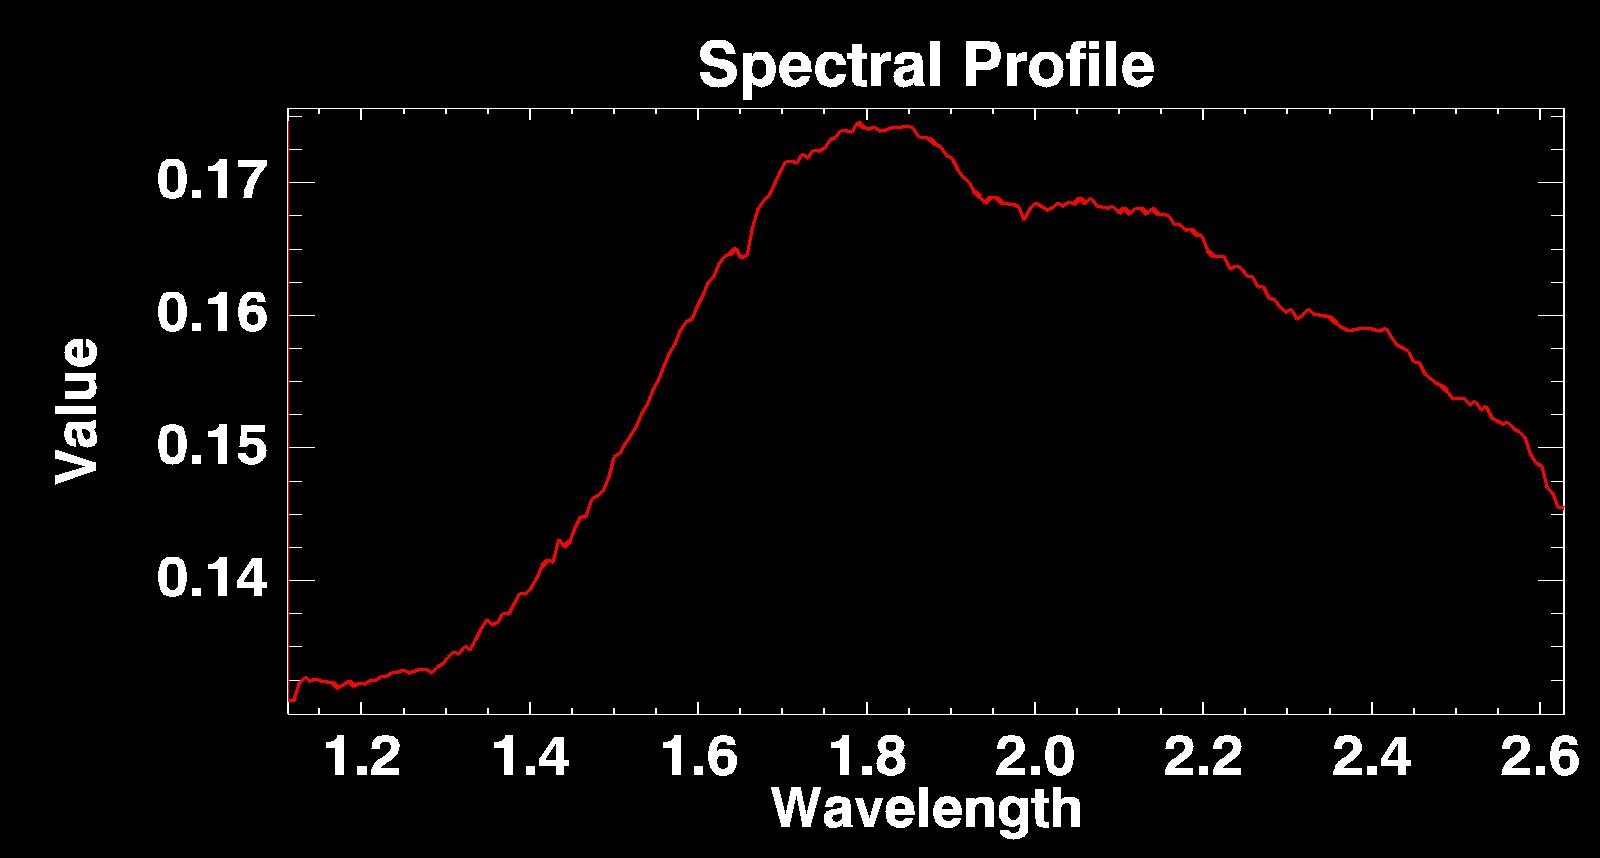
\includegraphics[width=\textwidth, height=1.5in]{dspkavgCorr3FB9_201_200.jpg}
                \caption{After final Despiking}
                \label{fig:dspkCorr_1}
        \end{subfigure}%
        ~ 
        
        \caption{Effect the column average correction and despiking for 3FB9 pixel at sample = 201 and line = 200.}
               
\end{figure*} 


\end{document}
